\section{Protocolos}

\begin{frame}{Protocolos}
	\begin{block}{Estructura Google Cast}
		\begin{itemize}
			\item Detección de dispositivos (mDNS)
			\item Intercambio de mensajes (Software propietario)
		\end{itemize}
	\end{block}
	
	\begin{block}{ }
		La primeras versiones del Chromecast usaban el protocolo DIAL que englobaba ambos pasos.		
	\end{block}
\end{frame}



\subsection{mDNS}

\begin{frame}{mDNS}
	\begin{block}{mDNS}
		Multicast Domain Name System es la implementación del protocolo de resolución de nombres (DNS) para redes de área local, donde no existe un servidor DNS real.		
	\end{block}
	
	\begin{block}{Ventajas}
		\begin{itemize}
			\item Poca configuracion para activarse
			\item Funciona cuando no hay infraestructura
			\item Soporta fallos en la infraestructura
		\end{itemize}
	\end{block}
\end{frame}


\begin{frame}{Primer paso mDNS}
	\begin{figure}[H]
		\centering
		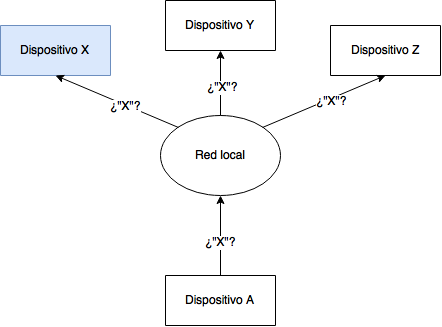
\includegraphics[width=0.75\textwidth]{./Imagenes/mdns1.png}
		\label{fig:mdns1}
		%\caption{Primer paso del protocolo mDNS}
	\end{figure}
\end{frame}

\begin{frame}{Segundo paso mDNS}
	\begin{figure}[H]
		\centering
		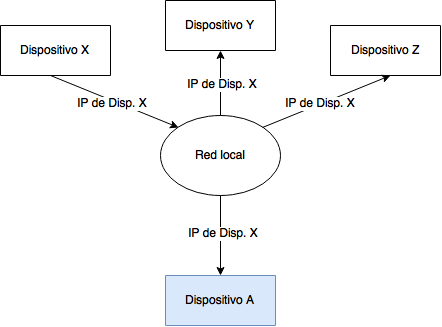
\includegraphics[width=0.75\textwidth]{./Imagenes/mdns2.png}
		\label{fig:mdns2}
		%\caption{Segundo paso del protocolo mDNS}
	\end{figure}
\end{frame}




\subsection{Comparación otros protocolos}

\subsubsection{Mirascat}

\begin{frame}{Miracast}
	\begin{block}{ }
		Miracast es un protocolo multimedia para hacer streaming a un monitor desde un dispositivo local.

		Con Miracast el dispositivo receptor es dependiente de que el dispositivo Android emisor se mantenga activo: si se bloquea también bloqueará la reproducción en el receptor.
	\end{block}
	
	\begin{block}{Capas}
		\begin{itemize}
			\item Capa de internet: IPv4
			\item Capa de transporte: TCP/UDP
			\item Capa de aplicación, RTSP y RTP
		\end{itemize}
	\end{block}
\end{frame}

\begin{frame}
	\begin{block}{Red}
		La conexión está creada vía Wi-Fi Protected Setup
		(WPS), mecanismos para facilitar la configuración de
		una red WLAN con seguridad WPA2.
		
		Existe una alternativa de código abierto a Miracast llamada \href{https://github.com/albfan/miraclecast}{MiracleCast}.
	\end{block}
	
	\begin{alertblock}{Sin soporte de Google}
		A partir de Android 6.0, Google ha dejado de dar soporte nativo a Miracast en favor de su propio Google Cast.
	\end{alertblock}
\end{frame}
